% !TEX program = pdflatex
% Options for packages loaded elsewhere
\PassOptionsToPackage{unicode}{hyperref}
\PassOptionsToPackage{hyphens}{url}
%
\documentclass[
]{article}
\usepackage{amsmath,amssymb}
\usepackage{lmodern}
\usepackage{iftex}
\ifPDFTeX
  \usepackage[T1]{fontenc}
  \usepackage[utf8]{inputenc}
  \usepackage{textcomp} % provide euro and other symbols
\else % if luatex or xetex
  \usepackage{unicode-math}
  \defaultfontfeatures{Scale=MatchLowercase}
  \defaultfontfeatures[\rmfamily]{Ligatures=TeX,Scale=1}
\fi
% Use upquote if available, for straight quotes in verbatim environments
\IfFileExists{upquote.sty}{\usepackage{upquote}}{}
\IfFileExists{microtype.sty}{% use microtype if available
  \usepackage[]{microtype}
  \UseMicrotypeSet[protrusion]{basicmath} % disable protrusion for tt fonts
}{}
\makeatletter
\@ifundefined{KOMAClassName}{% if non-KOMA class
  \IfFileExists{parskip.sty}{%
    \usepackage{parskip}
  }{% else
    \setlength{\parindent}{0pt}
    \setlength{\parskip}{6pt plus 2pt minus 1pt}}
}{% if KOMA class
  \KOMAoptions{parskip=half}}
\makeatother
\usepackage{xcolor}
\usepackage{longtable,booktabs,array}
\usepackage{calc} % for calculating minipage widths
% Correct order of tables after \paragraph or \subparagraph
\usepackage{etoolbox}
\makeatletter
\patchcmd\longtable{\par}{\if@noskipsec\mbox{}\fi\par}{}{}
\makeatother
% Allow footnotes in longtable head/foot
\IfFileExists{footnotehyper.sty}{\usepackage{footnotehyper}}{\usepackage{footnote}}
\makesavenoteenv{longtable}
\usepackage{graphicx}
\makeatletter
\def\maxwidth{\ifdim\Gin@nat@width>\linewidth\linewidth\else\Gin@nat@width\fi}
\def\maxheight{\ifdim\Gin@nat@height>\textheight\textheight\else\Gin@nat@height\fi}
\makeatother
% Scale images if necessary, so that they will not overflow the page
% margins by default, and it is still possible to overwrite the defaults
% using explicit options in \includegraphics[width, height, ...]{}
\setkeys{Gin}{width=\maxwidth,height=\maxheight,keepaspectratio}
% Set default figure placement to htbp
\makeatletter
\def\fps@figure{htbp}
\makeatother
\setlength{\emergencystretch}{3em} % prevent overfull lines
\providecommand{\tightlist}{%
  \setlength{\itemsep}{0pt}\setlength{\parskip}{0pt}}
\setcounter{secnumdepth}{-\maxdimen} % remove section numbering
\ifLuaTeX
  \usepackage{selnolig}  % disable illegal ligatures
\fi
\IfFileExists{bookmark.sty}{\usepackage{bookmark}}{\usepackage{hyperref}}
\IfFileExists{xurl.sty}{\usepackage{xurl}}{} % add URL line breaks if available
\urlstyle{same} % disable monospaced font for URLs
\hypersetup{
  hidelinks,
  pdfcreator={LaTeX via pandoc}}

\author{}
\date{}

\begin{document}

\textbf{TITLUL LUCRĂRII DE FINALIZARE A STUDIILOR}

\textbf{(Arial, 20 pt, Bold, Uppercase, Center)}

\textbf{Candidat: Prenume, Nume}

\textbf{(Arial 14 pt, Bold, Left)}

\textbf{Coordonator științific:
Asist.(SL/Lect./Conf./Prof.)dr.ing.(arh./ec./chim.) Prenume, Nume}

\textbf{(Arial 14 pt, Bold, Left)}

Sesiunea: Iunie 2022 (Arial 14 pt, Regular, Center)

\textbf{REZUMAT}

\textbf{(Arial 20 pt, Bold, Uppercase, Center)}

Rezumatul este destinat să informeze despre conținutul lucrării printr-o
scurtă descriere a cercetării de maximum o pagină, a
procedurilor/metodelor, precum și a rezultatelor sau concluziilor
acesteia. Rezumatul în limba română devine obligatoriu pentru lucrările
editate în alte limbi decât limba română și se va scrie cu caractere
Arial de 12 pt. Acesta va începe la două rânduri lăsate libere după
titlul „REZUMAT''. Înainte de titlu se vor lăsa libere trei linii de 12
pt.

\textbf{ABSTRACT}

\textbf{(Arial 20 pt, Bold, Uppercase, Center)}

The English abstract will be on the third page of the manuscript and
will present synthetically the paper work. The maximum length of the
abstract is one page written with Arial characters, size 12 pt. The
abstract text will begin after two blank lines (size 12pt.) from the
``ABSTRACT'' title. Before title there will be left three blank lines of
12pt size.

\hypertarget{introducere-14-pt-bold-uppercase-center}{%
\section{\texorpdfstring{\hfill\break
INTRODUCERE (14 pt, Bold, Uppercase,
Center)}{ INTRODUCERE (14 pt, Bold, Uppercase, Center)}}\label{introducere-14-pt-bold-uppercase-center}}

Fiecare capitol trebuie să aibă o structură clară, va începe pe pagină
nouă și va conține un titlu. Va fi urmat de două linii de 12 pt lăsate
libere.

\hypertarget{informaux163ii-generale-12-pt-bold-uppercase-left}{%
\subsection{INFORMAŢII GENERALE (12 pt, Bold, Uppercase,
Left)}\label{informaux163ii-generale-12-pt-bold-uppercase-left}}

Fiecare secțiune a unui capitol (ex. 1.1 INFORMAȚII GENERALE) va fi
poziționat la un rând liber sub text și va avea un rând liber de12 pt
deasupra textului.

Textul lucrării va fi aliniat uniform (justify). Este de preferat ca
textul să fie verificat pentru eventualele erori în limba de editare cu
ajutorul facilității de verificare a ortografiei (speller) din programul
word. Este recomandat ca lucrarea de finalizare a studiilor să nu
depășească 100 de pagini, inclusiv anexele.

Reguli aplicate pentru textul lucrării:

a. Marginile paginii -- se vor utiliza următoarele valori pentru
marginile paginii (Page Setup -\textgreater{} Margins-\textgreater{}
Mirror Margins):

- interior: 2 cm

- exterior: 2 cm

- sus: 2,5 cm (inclusiv header)

- jos: 2 cm

b. Spațiere între rânduri - textul va respecta o spațiere între rânduri
de 1,15 linii (Format\textgreater Paragraph-\textgreater Line
spacing-\textgreater{} 1,15 lines);

c. Alinierea textului în cadrul paragrafelor - textul din cadrul
paragrafelor normale va fi aliniat între marginile din stânga şi dreapta
(justified). Primul rând al fiecărui paragraf va avea o aliniere de 1,5
cm (Format-\textgreater{} Paragraph-\textgreater{}
Indentation-\textgreater{} Left). Excepție fac titlurile capitolelor,
care vor fi aliniate la stânga, precum și etichetele tabelelor și ale
figurilor (conform explicațiilor de mai jos);

d. Font -- fontul utilizat pentru redactare va fi Arial, cu dimensiunea
de 12 puncte, utilizând diacriticele specifice limbii în care este
redactată lucrarea (ex: ă, ş, ţ, î, â - pentru limba română);

e. Numerotarea paginilor - numerotarea paginilor se face începând cu
pagina de titlu, până la ultima pagină a lucrării, dar numărul paginii
apare doar începând cu Introducerea. Numărul de pagină se inserează în
subsolul paginii, centrat.

f. Antetul paginii -- apare începând cu introducerea și va conține pe
rânduri succesive un text cu înălțimea de 8, aliniat la stânga: (i)
textul Universitatea Politehnica Timișoara ; (ii) denumirea programului
de studii și anul susținerii ; (iii) numele candidatului (în stânga) și
titlul lucrării. În partea dreaptă a antetului poate fi integrată sigla
UPT;

\hypertarget{figuri-ux219i-fotografii-12-pt-bold-uppercase-left}{%
\subsection{\texorpdfstring{ FIGURI ȘI FOTOGRAFII (12 pt, Bold,
Uppercase,
Left)}{ FIGURI ȘI FOTOGRAFII (12 pt, Bold, Uppercase, Left)}}\label{figuri-ux219i-fotografii-12-pt-bold-uppercase-left}}

Figurile (incluzând imagini, grafice, capturi de ecran) se numerotează
în ordinea apariției în lucrare. Alternativ, figurile pot fi numerotate
în ordine în fiecare capitol, integrând în numerotare și numărul
capitolului. Fiecare figură are număr și titlu, care se menționează sub
figură, centrat. Dacă este cazul, sursa figurii se indică între
paranteze după titlul figurii. Toate figurile şi fotografiile prezentate
în lucrare trebuie să fie referite în textul lucrării, trebuie să fie
numerotate şi însoţite de titlul figurii.

Se va lăsa câte o linie liberă (Arial 12 pt) între figură şi text.
Figurile vor fi centrate pe pagină.

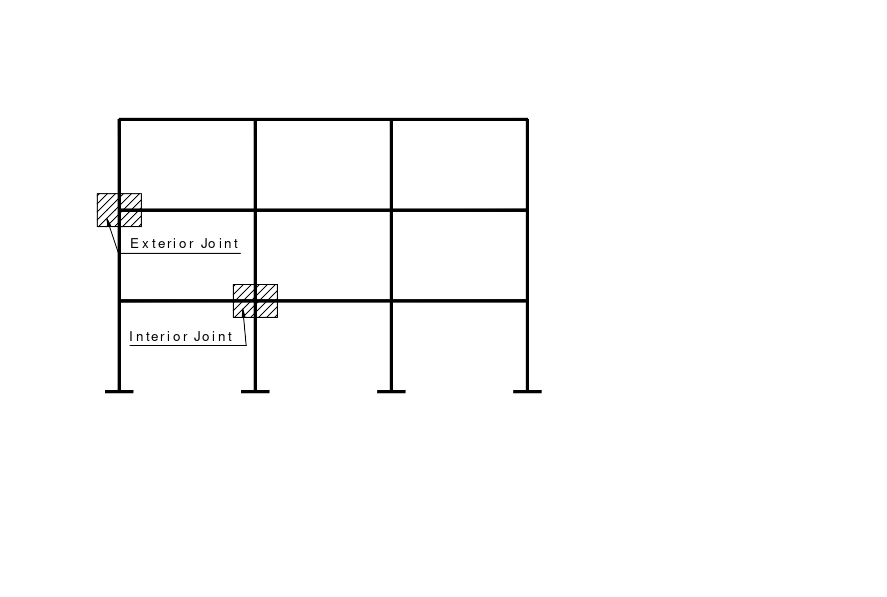
\includegraphics[width=3.95347in,height=2.55556in]{vertopal_7bfba83002a042659755220b13a52129/media/image1.png}

Figura 1 -- Exemplu de figură (sursa: Buletinul ştiinţific al UPT seria
construcţii-arhitectură nr.2 /2010)

\hypertarget{tabele-12-pt-bold-uppercase-left}{%
\subsection{TABELE (12 pt, Bold, Uppercase,
Left)}\label{tabele-12-pt-bold-uppercase-left}}

Tabele -- tabelele se numerotează în ordinea apariției în lucrare.
Alternativ, tabelele pot fi numerotate în ordine în fiecare capitol,
integrând în numerotare și numărul capitolului. Fiecare tabel are număr
și titlu, care se menționează deasupra tabelului, aliniat centrat. Dacă
este cazul, sursa datelor se precizează între paranteze după titlul
tabelului;

Toate tabelele prezentate în lucrare trebuie să fie referite în textul
lucrării, trebuie să fie numerotate şi însoţite de un titlu (vezi
exemplul de mai jos). Dacă se utilizează figuri copiate atunci se va
indica sursa fotografiei în paranteză. Pe cât posibil, în tabel se va
păstra fontul uzual (arial 12 pt) dar sunt acceptate şi modalităţi de a
scoate în evidenţă rezultatele importante (bold, italic etc.)

Se va lăsa câte o linie liberă (arial 12 pt) între text şi tabel.
Tabelele vor fi centrate pe pagină.

Tabelul 1. Exemplu de tabel

\begin{longtable}[]{@{}
  >{\raggedright\arraybackslash}p{(\columnwidth - 8\tabcolsep) * \real{0.2105}}
  >{\raggedright\arraybackslash}p{(\columnwidth - 8\tabcolsep) * \real{0.1973}}
  >{\raggedright\arraybackslash}p{(\columnwidth - 8\tabcolsep) * \real{0.1974}}
  >{\raggedright\arraybackslash}p{(\columnwidth - 8\tabcolsep) * \real{0.1974}}
  >{\raggedright\arraybackslash}p{(\columnwidth - 8\tabcolsep) * \real{0.1974}}@{}}
\toprule()
\endhead
&
\multicolumn{2}{>{\raggedright\arraybackslash}p{(\columnwidth - 8\tabcolsep) * \real{0.3947} + 2\tabcolsep}}{%
Yield stress, fy {[}N/mm2{]}} &
\multicolumn{2}{>{\raggedright\arraybackslash}p{(\columnwidth - 8\tabcolsep) * \real{0.3948} + 2\tabcolsep}@{}}{%
Tensile strength, fu {[}N/mm2{]}} \\
Element & Mill certificate & Coupon tests & Mill certificate & Coupon
tests \\
Beam IPE360 & 285.0 & 329.8 flange

348.4 web & 427.0 & 463.2 flange

464.0 web \\
Column HEB300 & 311.3 & 313.0 flange

341.8 web & 446.0 & 449.8 flange

464.4 web \\
End plate & 281.0 & 248.3 & 424.7 & 416.0 \\
Cover plate & 296.0 & 273.2 & 443.0 & 436.7 \\
\bottomrule()
\end{longtable}

\hypertarget{formulele-12-pt-bold-uppercase-left}{%
\subsection{\texorpdfstring{ FORMULELE (12 pt, Bold, Uppercase,
Left)}{ FORMULELE (12 pt, Bold, Uppercase, Left)}}\label{formulele-12-pt-bold-uppercase-left}}

Formulele utilizate în text se vor numerota în ordinea apariției în
lucrare. Alternativ, formulele pot fi numerotate în ordine în fiecare
capitol, integrând în numerotare și numărul capitolului. Numerotarea
formulelor se face în paranteze rotunde. Se va lăsa câte o linie liberă
(arial 12 pt) între text şi formulă. Formulele vor fi aliniate la
dreapta.

\begin{quote}
\(A = \pi r^{2}\) (1)
\end{quote}

\hypertarget{n.-concluzii-14-pt-bold-uppercase-center}{%
\section{N. CONCLUZII (14 pt, Bold, Uppercase,
Center)}\label{n.-concluzii-14-pt-bold-uppercase-center}}

Lucrarea se va încheia cu un capitol de concluzii. Acesta va conţine
principalele rezultate ale lucrării şi implicaţiile practice ale
acestora. În cazul proiectelor de diplomă, se vor menționa principalele
date sintetice obținute din procesul de proiectare

\hypertarget{bibliografie}{%
\section{BIBLIOGRAFIE}\label{bibliografie}}

La sfârşitul lucrării va fi dată o listă de referinţe pentru textele
ştiinţifice consultate pe parcursul realizării lucrării. Vor fi trecute
toate sursele, inclusiv cele de pe internet. Acestea vor fi referite în
text şi trecute în lista de referinţe în ordine alfabetică, după
exemplele de mai jos.

Bibliografia trebuie să cuprindă toate titlurile din literatura de
specialitate care au servit ca bază de documentare, respectiv autorii
care au fost citați în text, la toate capitolele lucrării. Facultățile
pot adopta sisteme de citare proprii în concordanță cu specificul
domeniilor coordonate.

În lipsa unor cerințe de citare impuse, bibliografia va fi redactată
conform normelor Academiei Române.

În textul lucrării referințele vor fi referite în paranteze, spre
exemplu (Tremblay, 2002).Referințele vor fi menționate în limba în care
au fost consultate (nu vor fi traduse).

Lista bibliografică va fi aranjată în ordine alfabetică, a primului
autor. În cazul în care avem două sau mai multe lucrări scrise de
același autor acestea vor fi trecute în ordine cronologică. Referințele
vor include:

\begin{itemize}
\item
  numele autorului, prenumele, titlul - scris cu Italic - volumul,
  localitatea, editura, anul;
\item
  pentru un studiu sau o publicație periodică se trec numele și
  prenumele autorului, titlul articolului - scris cu Italic - numele
  publicației, anul de apariție a seriei, seria, numărul, anul
  calendaristic.
\end{itemize}

Sursele bibliografice, publicate sau nepublicate trebuie să se
regăsească în lista bibliografică finală, după cum toți autorii incluși
în lista bibliografică trebuie să fie inserați în textul lucrării.

Preluarea identică a unei fraze sau paragraf va fi citată prin indicarea
inclusiv a paginii din sursa utilizată, dar și prin ghilimele şi forma
italică a literelor; pentru sursele preluate de pe internet, vor fi
notate adresele de pagină web; în lista bibliografică finală lucrările
se trec în ordinea alfabetică a numelor autorilor. La lucrările
colective, regula referitoare la ordinea alfabetică este valabilă pentru
primul autor.

Dacă se citează site-uri web, reviste sau articole, înainte de acestea
se vor trece trei asteriscuri, informații referitoare la volum, număr,
pagini consultate, adresa web exactă a articolului respectiv, data
vizitării site-ului și a descărcării materialului, data accesării.
Adresele de pagini web se regăsesc la finalul listei.

Sursele bibliografice la care nu se poate menționa autorul se vor
specifica astfel: „***''urmat de denumirea articolului și/sau a cărții,
editura și locul apariției (pentru cărți), volumul, numărul acestuia,
prima și ultima pagină a lucrării citate, anul apariției.

Sursele bibliografice consultate pe Internet se vor specifica astfel:
pagina care a fost consultată, data ultimei accesări. Este recomandat să
se alăture link-ul către pagina respectivă de internet. Notele și
trimiterile bibliografice se trec la sfârșitul capitolului/lucrării, în
ordinea în care apar în text; acolo unde este inserată nota sau
trimiterea bibliografică, la ultimul cuvânt se marchează numărul
acesteia, la exponent, cu cifre arabe; la subsol sau la sfârșitul
capitolului se trece conținutul notei, respectiv trimiterii
bibliografice, după cerințele menționate.

Exemple de referințe:

Coulouris, G., Dollimore, J., Kindberg, T., \emph{Distributed systems,
concepts and design}, 3rd edition, Pearson, Addison Wesley, 2001.

Tremblay, R., \emph{Inelastic seismic response of steel bracing
members,} Journal of Constructional Steel Research, 58, pp 665--701,
2001.

Neculau, A., Cozma, T. (coord.), Psiho -pedagogie - pentru examenul de
definitivat şi gradul II, Iaşi, Editura Spiru Haret, 1994.

*** https://ro.wikipedia.org/wiki/Motor\_cu\_reac\%C8\%9Bie accesare
februarie 2022)

Ultima pagină a lucrării de disertație trebuie să conțină „Declarația de
originalitate a lucrării de finalizare a studiilor'', completată
olograf, în conformitate cu cerinţele UPT. Declaraţia se descarcă de pe
adresa de web:

\url{http://www.upt.ro/pdf/licenta\&master/Declaratie_de_autenticitate_UPT.pdf}

\end{document}
